\documentclass[border=0]{standalone}
\usepackage{booktabs}
\usepackage{tikz}

\usetikzlibrary{positioning}

\begin{document}
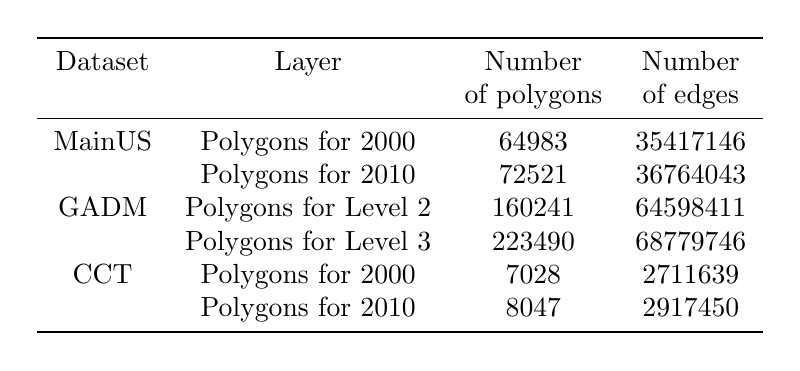
\begin{tikzpicture}
    \node[] (vertices) at (0,0) {
        \begin{tabular}{c c c c}
            \toprule
            Dataset & Layer & Number        & Number    \\
                    &       & of polygons   & of edges  \\
            \midrule
            MainUS& Polygons for 2000 & 64983 & 35417146        \\
                & Polygons for 2010 & 72521 & 36764043        \\
            GADM  & Polygons for Level 2 & 160241 & 64598411    \\
                & Polygons for Level 3 & 223490 & 68779746    \\
            CCT   & Polygons for 2000 & 7028 & 2711639          \\
                & Polygons for 2010 & 8047 & 2917450          \\
            \bottomrule
        \end{tabular}
    };
\end{tikzpicture}
\end{document}
